

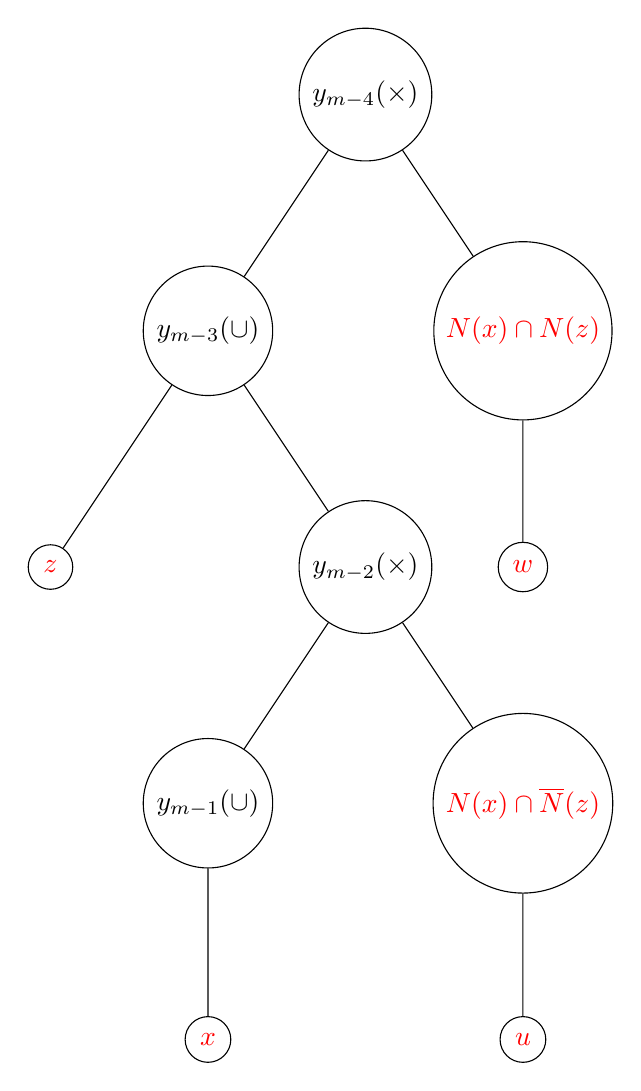
\begin{tikzpicture}[every node/.style={circle,draw,minimum size=5mm},level distance=3cm,
  level 1/.style={sibling distance=4cm},
  level 2/.style={sibling distance=2cm}
  level 3/.style={sibling distance=3cm}
  ]
    
    \node {$y_{m-4}(\times)$}
        child{ node {$y_{m-3}(\cup)$}
                 child { node {\textcolor{red}{$z$} }}
                 child { node {$y_{m-2}(\times)$}
                    child { node {$y_{m-1}(\cup)$}
                         child { node {\textcolor{red}{$x$} }}
                    }
                    child { node {\textcolor{red}{$N(x) \cap \overline{N}(z)$} }
                         child { node {\textcolor{red}{$u$} }}
                    }
                 }
        }
         child { node {\textcolor{red}{$N(x) \cap N(z)$} }
                         child { node {\textcolor{red}{$w$} }}
                    }
        ;
\end{tikzpicture}